\documentclass{../lista}

\begin{document}
	\cabecalhoAlt
	{Simulado | 2º Intensivo para a OBA}
	{Questões}
	{Gabriel Lucena e Iago Mendes}

	\begin{secao}{Questões de Astronomia}
		% 1
		\begin{questao}{(1 ponto)}
			Some a pontuação de cada item verdadeiro: \\
			
			1. Um observador do hemisfério norte e um observador do hemisfério sul observam a mesma fase da Lua, mas com a imagem invertida
			
			2. O lado oculto da Lua nunca recebe energia do Sol
			
			4. Nós sempre observamos exatamente o mesmo lado da Lua 
			
			8. A Lua Quarto-Minguante nasce ao meio-dia
			
			16. A Lua Quarto-Crescente se põe à meia noite
			
			\begin{alternativas}
				\item 10
				\item 17
				\item 18
				\item 20
			\end{alternativas}
			
		\end{questao}

		% 2
		\begin{questao}{(1 ponto)}
			Qual dos seguintes anos \textbf{NÃO} é um ano bissexto?
			
			\begin{alternativas}
				\item 1956
				\item 2000
				\item 2280
				\item 2300
			\end{alternativas}
		\end{questao}

		% 3
		\begin{questao}{(1 ponto)}
			Substitua os nomes dos respectivos astrônomos na ordem correta:
			
			1. O modelo geocêntrico que a Terra se encontra no centro do sistema solar foi proposto por \textbf{nome 1}.
			
			2. \textbf{nome 2} determinou o raio da Terra com medições na cidade de Alexandria e Syene.
			
			3. \textbf{nome 3} propôs o modelo heliocêntrico que o Sol está no centro do sistema solar.
			
			4. \textbf{nome 4} desenvolveu um catálogo de observações astronômicas mais preciso da época, apesar de apoiar o modelo geocêntrico.
			
			\begin{alternativas}
				\item Tycho Brahe - Erastóstenes - Copérnico - Ptolomeu
				\item Erastóstenes - Ptolomeu - Copérnico - Tycho Brahe
				\item Copérnico - Ptolomeu - Erastóstenes - Tycho Brahe
				\item Ptolomeu - Erastóstenes - Copérnico - Tycho Brahe
			\end{alternativas}
		\end{questao}

		% 4
		\begin{questao}{(1 ponto)}
			\begin{center}
				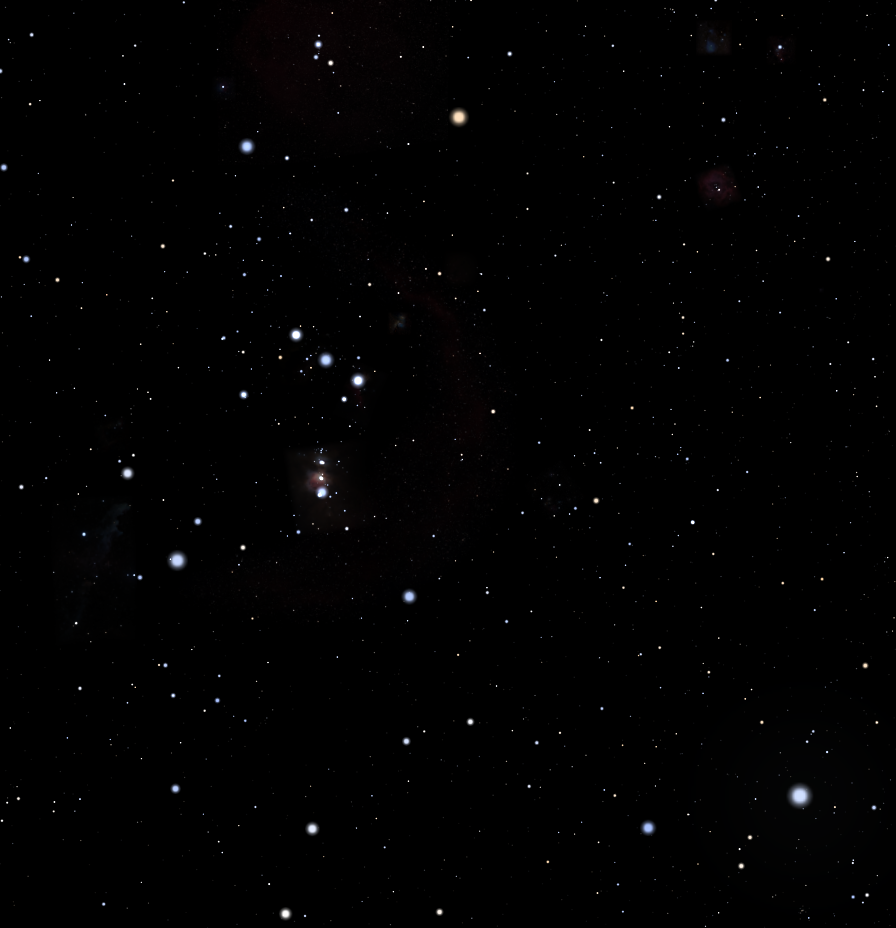
\includegraphics[height=.75\linewidth]{./img/4.png}
			\end{center}
			
			Some a pontuação para cada um dos itens verdadeiros:
			
			1. A estrela mais brilhante do céu noturno está visível
			
			2. A Grande Nebulosa de Órion está no campo de visão da foto
			
			4. A imagem está completamente no hemisfério sul
			
			8. As estrelas Beteulgeuse e Rigel fazem parte da constelação do Órion
			
			16. A estrela Sírius sempre foi a estrela mais brilhante do céu noturno.
			
			\begin{alternativas}
				\item 7
				\item 11
				\item 18
				\item 20
			\end{alternativas}
		\end{questao}

		% 5
		\begin{questao}{(1 ponto)}
			A seguir temos algumas relações, some a pontuação de cada uma das relações verdadeiros: \\
			
			1. A Terra rotaciona do Oeste para o Leste $\rightarrow$ Sol nasce no Leste e se põe no Oeste.
			
			2. O Sol está no ponto de Áries $\rightarrow$ O Sol está saindo do hemisfério sul e entrando no hemisfério norte.
			
			4. A órbita lunar possui é uma elipse $\rightarrow$ Efeito de libração longitudinal
			
			8. A órbita lunar é inclinada em relação à eclíptica $\rightarrow$ Efeito de libração latitudinal
			
			16. O movimento de precessão $\rightarrow$ A estrela polar de cada hemisfério nunca mudam
			
			\begin{alternativas}
				\item 11
				\item 15
				\item 20
				\item 31
			\end{alternativas}
		\end{questao}

		% 6
		\begin{questao}{(1 ponto)}
			O Sol tem, aproximadamente, o mesmo tamanho angular da Lua. Sabendo que a distância da Terra ao Sol é 388 vezes maior que a distância da Terra à Lua e o raio da Lua vale $1740 \; km$, qual o tamanho do diâmetro do Sol?
			
			\begin{alternativas}
				\item $675120 \; km$
				\item $337560 \; km$
				\item $1350240 \; km$
				\item $4050720 \; km$
			\end{alternativas}
		\end{questao}

		% 7
		\begin{questao}{(1 ponto)}
			Um satélite geoestacionário é um satélite que possui período orbital igual ao período de rotação da Terra. Calcule a \textbf{altura aproximada} da órbita geoestacionária em relação à superfície da Terra. Utilize a terceira lei de Kepler e os seguintes dados:
			
			\begin{equation}
				M_{Terra} = 6 \cdot 10^{24} \; kg \\
				G = 6.67 \cdot 10^{-11} \; N m^{2} / kg^{2} \\
				R_{Terra} = 6371 \; km
			\end{equation}
			
			\begin{alternativas}
				\item $48680 \; km$
				\item $42300 \; km$
				\item $35900 \; km$
				\item $29500 \; km$
			\end{alternativas}
		\end{questao}
	\end{secao}

	\begin{secao}{Questões de Astronáutica}
		% 8
		\begin{questao}{(1 ponto) [OBA 2008 Adaptada]}
			Uma empresa privada dos EUA está desenvolvendo um avião espacial (SpaceShipTwo) no qual turistas viajarão ao espaço em um vôo suborbital de 15 a 20 minutos. Durante a fase do vôo fora da atmosfera da Terra os turistas conseguirão ver a Terra da mesma forma que os astronautas a vêem em seus vôos orbitais e da Estação Espacial Internacional. Conforme mostrado na imagem ao lado, obtida do espaço, é possível ver claramente a curvatura da Terra (Aparentemente a Terra não é plana!). Analisando a imagem e usando a geometria e trigonometria que você aprendeu na escola é possível estimar a altitude da qual ela foi tirada. Neste caso, o comprimento estimado para o campo de visão horizontal é de 1.200 km.
			
			\begin{center}
				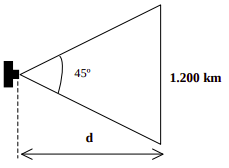
\includegraphics[height=.4\linewidth]{./img/8-1.png} 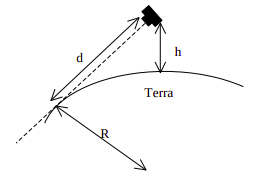
\includegraphics[height=.4\linewidth]{./img/8-2.png}
			\end{center}
			
			a) Com o uso da trigonometria podemos determinar outras informações a partir da imagem. Sabendo-se que o ângulo de visão da câmara fotográfica é de 45 graus na horizontal, determine a distância \textbf{d} do astronauta que tirou a foto até o horizonte da Terra. \\
			
			b) A distância d de um ponto qualquer acima da superfície da Terra até o horizonte é dada por $d = \sqrt{2 R h + h^{2}}$, onde R é o raio da Terra e h a altura onde foi feita a imagem. Determine a altura h da órbita de onde foi feita a imagem acima. Use a distância d obtida no item anterior. Utilize a calculadora para qualquer cálculo.
			
			\begin{alternativas}
				\item a. $1500 \; km$ e b. $300 \; km$
				\item a. $1200 \; km$ e b. $174 \; km$
				\item a. $1500 \; km$ e b. $174 \; km$
				\item a. $1200 \; km$ e b. $300 \; km$
			\end{alternativas}
		\end{questao}

		% 9
		\begin{questao}{(1 ponto) [OBA 2016 Adaptada]}
			De uma maneira simplificada um satélite de sensoriamento remoto pode ser entendido como uma “máquina fotográfica” que, do espaço, obtém imagens da Terra. A partir dessas imagens é possível monitorar e medir vários fenômenos que ocorrem na superfície terrestre, incluindo queimadas e desmatamento. É importante ressaltar, contudo, que a identificação das queimadas é feita a partir da captação da energia emitida pelo material orgânico em chamas, que ocorre, principalmente na faixa de comprimento de ondas entre 3,7µm e 4,1µm (1 µm = 10-6 m) do espectro eletromagnético, conhecida como termal-média. Sabe-se que quanto maior a temperatura da chama, maior é a emissão de energia. O desmatamento, por sua vez, é identificado a partir da radiação solar refletida em uma faixa de comprimento de onda entre 0,4 µm e 3,0 µm. Ao se analisar a radiação solar refletida pelos tipos de superfície nos diversos comprimentos de onda da radiação solar observa-se que a água (rios, lagos e mares) reflete menos energia solar quando comparada ao solo sem cobertura vegetal e ao solo com cobertura vegetal. Além disso, o solo exposto e a vegetação refletem diferentemente em todos os comprimentos de onda, o que permite sua diferenciação. Por se tratarem de fenômenos físicos distintos (emissão e reflexão) o satélite precisa possuir mais de uma câmera imageadora para monitorar o desmatamento e as queimadas. De modo similar a uma máquina fotográfica digital, as imagens obtidas pelos sensores de um satélite são transformadas em píxeis. Cada imagem é composta de milhões de píxeis. O pixel é o menor elemento da imagem, ao qual é possível atribuir uma tonalidade, cujo valor numérico varia entre zero e 255. Um pixel com valor zero significa que ele recebeu quase nenhuma radiação proveniente da superfície terrestre, sendo então representado pela cor preta. No outro extremo o valor 255 corresponde à cor branca e indica que o sensor recebeu a máxima quantidade de radiação da superfície terrestre. Entre zero e 255 há 254 tons de cinza do mais claro ao mais escuro. O normal é uma imagem com píxeis de diversas tonalidades de cinza, da mais clara (tendendo ao branco) à mais escura (tendendo ao negro). \\
			
			A partir dessas informações, some a pontuação em cada uma das seguintes sentenças: \\
			
			1. A partir de variações de tonalidade de cinza obtidas nas imagens dos satélites, os cientistas identificam regiões de queimadas e de desmatamento
			
			2. A presença de nuvens não atrapalha a detecção de queimadas e de desmatamento.
			
			4. Uma área queimada, depois do fogo extinto, irá refletir mais radiação solar do que antes, quando havia cobertura vegetal, e por isso, será representada por “píxeis” claros
			
			8. Quanto maior a temperatura da área sendo queimada, mais claros serão os píxeis que representam a imagem dessa área.
			
			16. Muitos píxeis de uma imagem de uma câmera satelital, destinada ao monitoramento de queimadas, apresentam valores numéricos próximos de 255. Isso significa a detecção de uma queimada.
			
			\begin{alternativas}
				\item 4
				\item 9
				\item 17
				\item 25
			\end{alternativas}
		\end{questao}

		% 10
		\begin{questao}{(1 ponto) [OBA 2018 Adaptada]}
			Com o desenvolvimento da astronáutica está cada vez mais fácil colocarmos telescópios em órbita. Contudo, alguns, como o SOHO (Solar and Heliospheric Observatory = Observatório Solar e Heliosférico), precisam girar ao redor do Sol no mesmo período que a Terra e ficar entre o Sol e a Terra, pois precisa observar o Sol 24h/dia. Mas pela terceira lei de Kepler , ou seja, quanto menor a distância ao Sol, menor será o período e viceversa. Logo, não seria possível colocar o SOHO e outros satélites para girarem ao redor do Sol, com o mesmo período da Terra estando num lugar diferente da Terra. Mas o italiano JosephLouis de Lagrange, em 1772, descobriu que há cinco pontos, chamados pontos Lagrangianos, num sistema Terra-Sol, ou Terra-Lua, ou Solplaneta, que são “especiais”. O ponto L1 fica na linha Terra-Sol, entre Terra e Sol e um observatório ali colocado move-se com o mesmo período da Terra, tal com faz o SOHO, o qual nunca é eclipsado pela Lua e recebe sempre a mesma irradiação do Sol. Veja a figura ao lado. O ponto L2 fica depois do cone de sombra (umbra) da Terra, será o local de posicionamento do Telescópio Espacial James Webb e terá período de translação igual ao da Terra. Os pontos L4 e L5 ficam sobre a órbita da Terra e são localizados por um triângulo equilátero com aresta igual à distância Terra-Sol.
			
			\begin{center}
				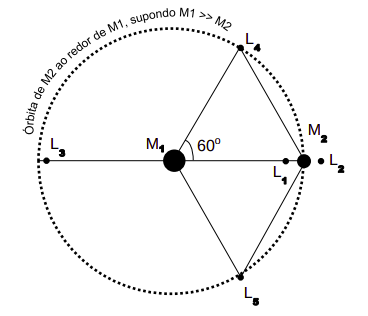
\includegraphics[height=.75\linewidth]{./img/10.png}
			\end{center}
			
			a) Considere que M1 seja a massa do Sol, M2 a massa da Terra, R a distância Terra-Sol e r a distância da Terra aos pontos Lagrangianos L1 e L2 (são simétricos em relação a M2). Pode-se demonstrar que r é dado por: $ r = \sqrt[3]{\frac{M_{1}}{3 M_{2}}} R = 1.4784 \cdot 10^{8} \; km$. Sabendo que a distância média à Lua é de $384000 \; km$, calcule quantas vezes $r$ está mais distante que a órbita da Lua.
			
			b) Conforme explicado, a vantagem dos pontos L1, L2 e L3 é que mesmo
			estando à diferentes distâncias da Terra ao Sol, ainda assim, satélites ali colocados teriam o mesmo período de translação da Terra ao redor do Sol, isto é, 365,25 dias. Qual seria o período de translação de satélites colocados nos pontos Lagrangianos L4 e L5?
			
			\begin{alternativas}
				\item a) 200 b) Metade do período da Terra
				\item a) 385 b) Metade do período da Terra
				\item a) 200 b) O mesmo período da Terra
				\item a) 385 b) O mesmo período da Terra
			\end{alternativas}
			
		\end{questao}
	\end{secao}

	\begin{secao}{Questões Avançadas}
		% 11
		\begin{questao}{(1 ponto)}
			Um fenômeno muito conhecido é o da ``laçada de Marte", em que o planeta Marte subitamente muda sua direção de deslocamento no céu, e quando acompanhado por vários dias parece se locomover formando um laço no céu.
			
			\begin{pergunta}{(1 ponto)}
				Quais planetas, além de Marte, reproduzem o mesmo fenômeno de modo que possamos observá-los em uma noite de céu limpo?
				
				\begin{multicols}{3}
					\begin{alternativas}
						\item[$(\quad)$] Mercúrio
						\item[$(\quad)$] Vênus
						\item Júpiter
						\item Saturno
						\item Urano
						\item Netuno
					\end{alternativas}
				\end{multicols}
			\end{pergunta}
		\end{questao}
		
		% 12
		\begin{questao}{(1 ponto) [USAAAO 2021 adaptada]}
			O cometa C/2020 F3 (NEOWISE) atingiu o periélio pela última vez em 3 de julho de 2020. O cometa NEOWISE tem um período orbital de $\approx 4.400$ anos e sua excentricidade é de $0,99921$.
			
			\begin{pergunta}{(1 ponto)}
				Qual é a distância do periélio do cometa NEOWISE, em $UA$?
				
				\begin{alternativas}
					\item $0,0123 \; UA$
					\item $0,212 \; UA$
					\item $2,69 \; UA$
					\item $26,8 \; UA$
				\end{alternativas}
			\end{pergunta}
		\end{questao}
		
		% 13
		\begin{questao}{(1 ponto)}
			Deneb é uma estrela de tipo espectral A2 cuja magnitude aparente na banda V é de 1,25. Certa noite Deneb se divide em 2 novas estrelas com a mesma temperatura da inicial. \\ \\
			Dado: \\
			$\log(2) \approx 0,3$
			
			\begin{pergunta}{(1 ponto)}
				Qual a nova magnitude aparente na banda V do sistema?
				
				\begin{alternativas}
					\item $1,25$
					\item $2,5$
					\item $1,0$
					\item $2,0$
				\end{alternativas}
			\end{pergunta}
		\end{questao}
		
		% 14
		\begin{questao}{(1 ponto) [USAAAO 2020 adaptada]}
			Em abril de 2020, o \textit{Event Horizon Telescope} divulgou a primeira imagem do buraco negro supermassivo da galáxia \textit{M87}. O buraco negro tem um diâmetro de aproximadamente $270 \; UA$ e está localizado a uma distância de $16,4 \; Mpc$.
			
			\begin{pergunta}{(1 ponto)}
				No comprimento de onda observado de $1,3 \; mm$, qual é a linha de base mínima aproximada, ou diâmetro efetivo, necessária para a imagem do buraco negro?
				
				\begin{alternativas}
					\item $2 \cdot 10^3 \; km$
					\item $2 \cdot 10^4 \; km$
					\item $2 \cdot 10^5 \; km$
					\item $2 \cdot 10^6 \; km$
					\item $2 \cdot 10^7 \; km$
				\end{alternativas}
			\end{pergunta}
		\end{questao}
		
		% 15
		\begin{questao}{(1 ponto) [Seletiva OBA Presencial 2016-17 adaptada]}
			A paralaxe heliocêntrica de Canopus, segundo os dados do satélite Hipparcos, vale $10,42$ milisegundos de arco ($mas$). \\ \\
			Dado: magnitude aparente de Canopus = $-0,72$
			
			\begin{pergunta}{(0,5 ponto)}
				Utilize essa informação e o módulo da distância para calcular a magnitude absoluta de Canopus.
				
				\begin{alternativas}
					\item $M = -5,63$
					\item $M = -0,72$
					\item $M = -1,44$
					\item $M = -2,82$
				\end{alternativas}
			\end{pergunta}
			
			\begin{pergunta}{(0,5 ponto)}
				Aproximadamente, quantas vezes ela é mais luminosa do que o Sol? \\
				Dado: magnitude absoluta do Sol = $+4,80$
				
				\begin{alternativas}
					\item $\approx 15$ mil vezes
					\item $\approx 30$ mil vezes
					\item $\approx 5$ mil vezes
					\item $\approx 50$ mil vezes
				\end{alternativas}
			\end{pergunta}
		\end{questao}
	\end{secao}
\end{document}